% Generated by GrindEQ Word-to-LaTeX 2008 
% ========== UNREGISTERED! ========== Please register! ==========
% LaTeX/AMS-LaTeX

\documentclass[a4paper]{article}
\usepackage{anysize}
\marginsize{1cm}{1cm}{1cm}{1cm}

\usepackage{amssymb}
\usepackage{amsmath}
\usepackage[pdftex]{graphicx}
\usepackage{epsfig}
\usepackage{subfigure}
\usepackage{listings}
\lstset{language=haskell}
\lstset{commentstyle=\textit}
\lstset{mathescape=true}
%\lstset{labelstep=1}
%\lstset{backgroundcolor=,framerulecolor=}
\lstset{backgroundcolor=,rulecolor=}
\linespread{2.0}

\begin{document}

%%% remove comment delimiter ('%') and select language if required
%\selectlanguage{spanish} 

\noindent 
\section{Concrete Subtyping}

\noindent The downcasting operation that would allow us to safely use references that expect a smaller heap in a context where a larger heap is available requires some preliminary work. 

\noindent First of all let us understand what kind of operation we will perform whenever we try to use a heap $h$ that is too large with respect to the get or set functions of the reference:

\begin{enumerate}
\item  We downcast the larger heap to an adequately smaller one

\item  We perform our computation on the downcast heap, thereby obtaining a new smaller heap

\item  We store the new smaller heap in the corresponding locations of the original heap
\end{enumerate}

\noindent The three steps listed above are summarized in the following diagram:

\begin{figure}[h]
\centerline{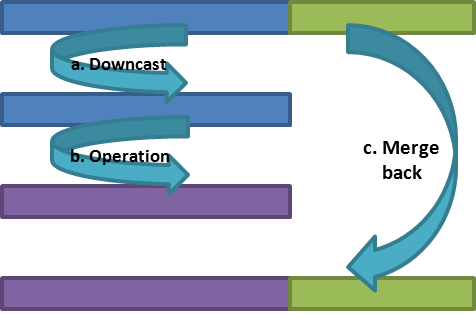
\psfig{file=heap_upcasting.png,height=5cm}} \caption{An example of picture.\label{fig:example}}
\end{figure}

\noindent The downcast operation is implemented easily enough on heaps thanks to the transitivity of the subtyping relationship. We just need to specify that:


\begin{lstlisting}
New h $\alpha$ $\le$ h
downcast=delete
\end{lstlisting}

And the first step of the computation is covered. Now we define the in-place substitution operation with an appropriate predicate:

\begin{lstlisting}
HList h $\wedge$ HList $h'$ $\wedge$ $h'$ $\le$ h $\Rightarrow$ InPlaceSubstitute h h'
    inPlaceSubstitute : h $\to$ $h'$ $\to$ $h'$
\end{lstlisting}

This new predicate is instanced inductively on the length of the prefix$\ h$:

\begin{lstlisting}
InPlaceSubstitute Nil h
    inPlaceSubstitute Nil h = h
\end{lstlisting}

and

\begin{lstlisting}
InPlaceSubstitute (h::tl) ($h'$::$tl'$)
    inPlaceSubstitute (h::tl) ($h'$::$tl'$) = h::(inPlaceSubstitute tl $tl'$)
\end{lstlisting}

Thanks to this new operator, which we could consider an upcasting operator of sorts, we can now define the proper downcasting operation for references:

\begin{lstlisting}[frame=tb,mathescape]{somecode}
HList h,HList $h'$, h $\le$ $h'$ $\Rightarrow$ Reference $h'$ $\alpha\le$ Reference $\alpha$
downcast (Reference get set)=Reference
		($\lambda$h.upcast h (get (downcast h)))
		($\lambda$v.$\lambda$h.upcast h (set v (downcast h)))
	where upcast h (x,$h'$) = (x, inPlaceSubstitute $h'$ h)
\end{lstlisting}

This operation invokes the get and set functions of a reference with the downcast (smaller) heap with respect to the input (larger) heap, and then rebuilds a larger heap by stitching together the input heap with the resulting heap from the get or set operation.

\noindent 

\end{document}

% == UNREGISTERED! == GrindEQ Word-to-LaTeX 2008 ==

